% Partie controleurs de jeu

\subsection{Cas d'utilisation}

	\subsubsection{Navigation dans le menu}
	Le joueur peut agir sur le menu par l'intermédiaire des contrôleurs de jeu et peut ainsi effectuer quatre actions distincts représentées par le diagramme de cas d'utilisation ci-dessous. Cependant le cas d'utilisation "Saisir du texte" n'est disponible que lors de l'utilisation d'un clavier.
	
		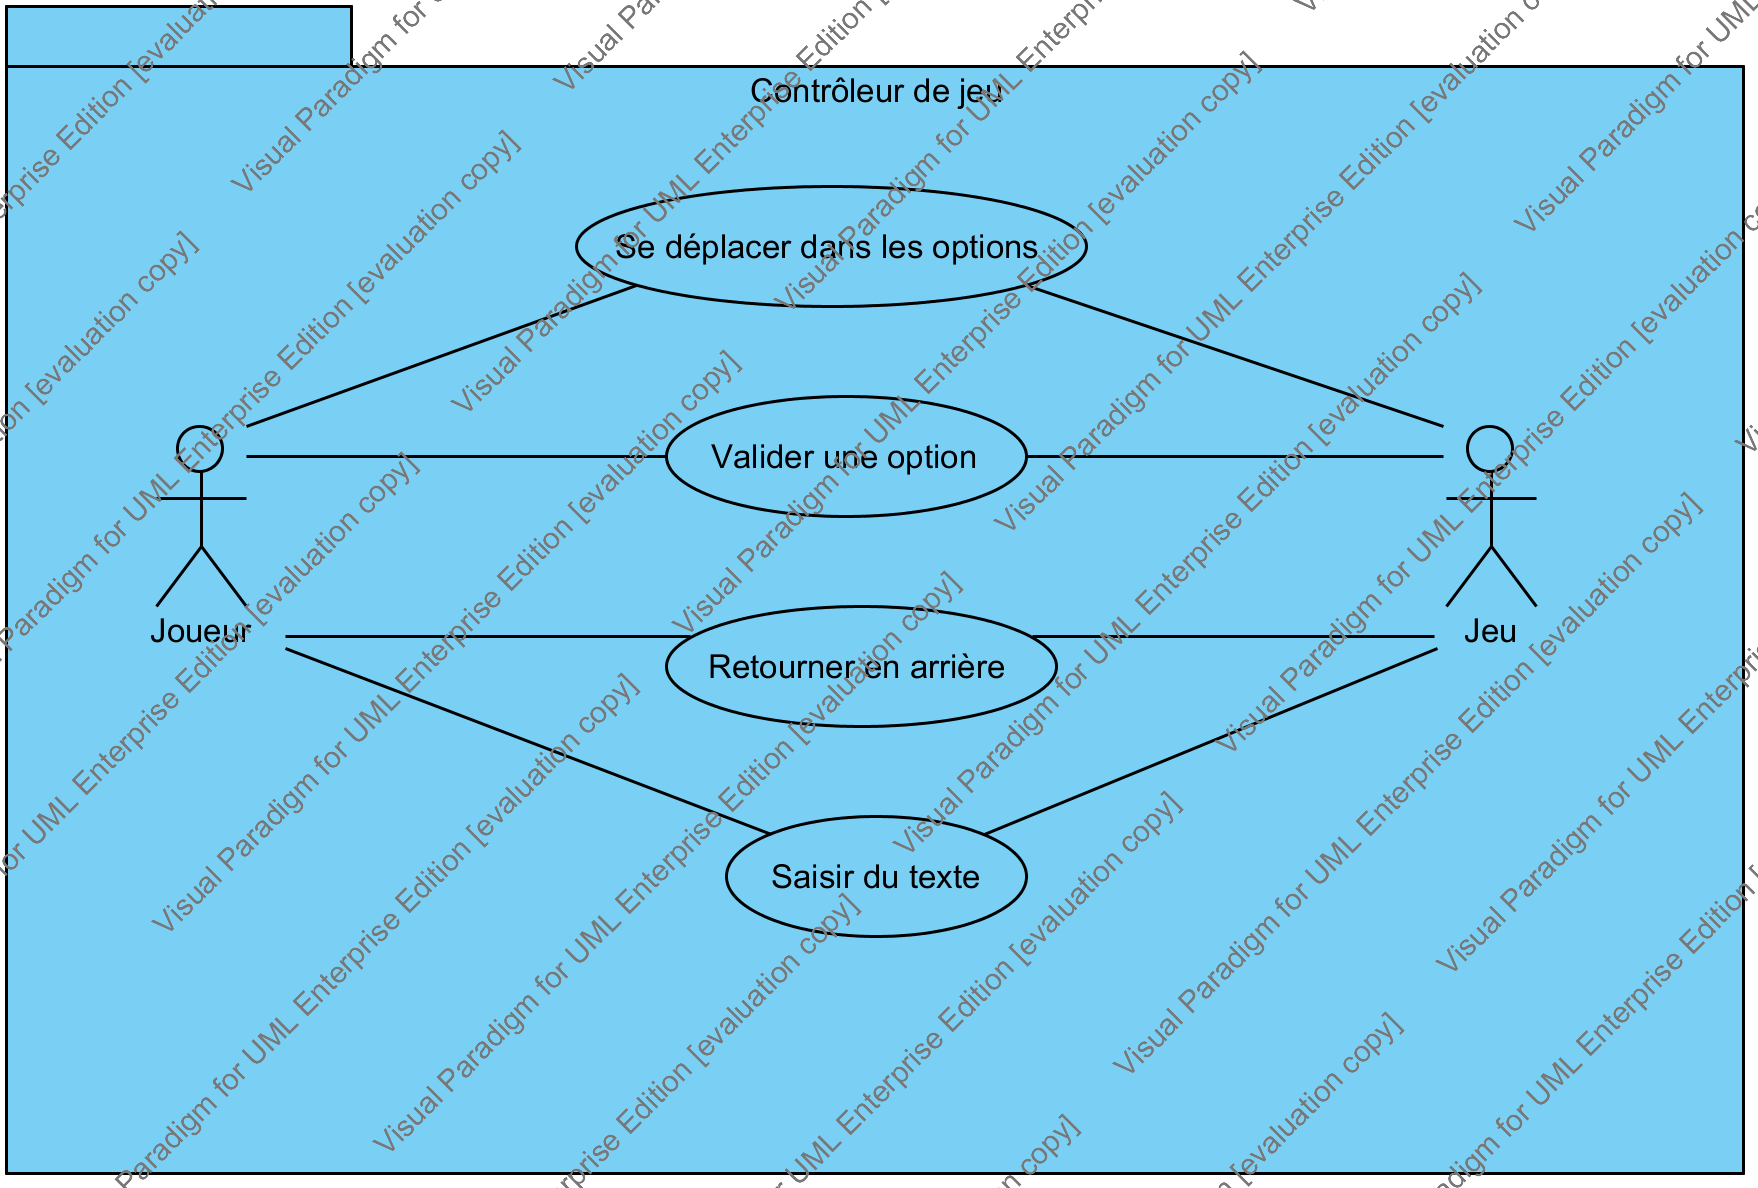
\includegraphics{images/UML/UseCase/controller_navigMenu}
				
		
	\subsubsection{Navigation dans le jeu}
	Durant la phase de jeu, chaque joueur peut réaliser six actions lesquelles sont définies par le diagramme suivant :
	
		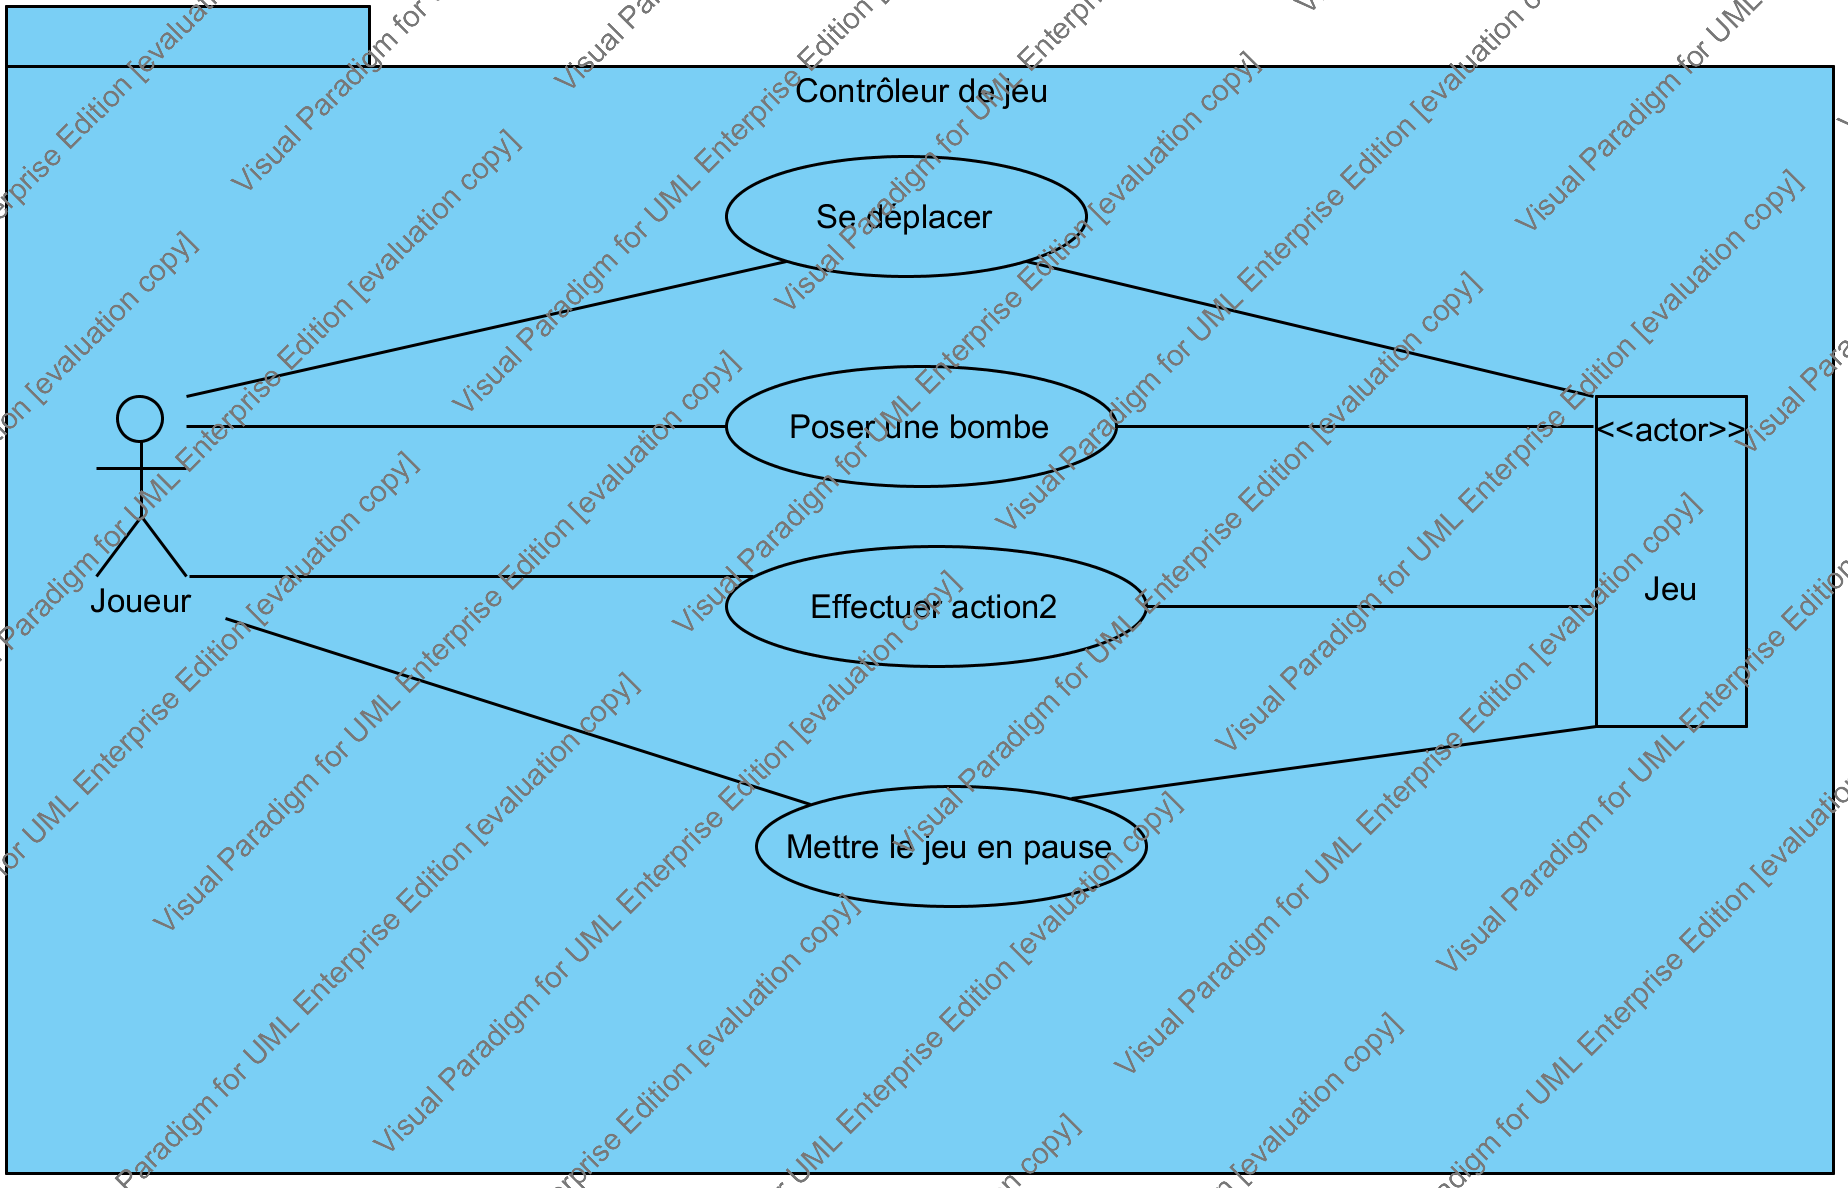
\includegraphics{images/UML/UseCase/controller_gameActions}
	
\subsection{Diagramme de classes}

La communication entre le menu et les contrôleurs s'effectue par l'intermédiaire de l'interface IControllerToMenu. Le menu est contrôlable par l'intermédiaire d'un objet de type Controller qui est soit un clavier, soit un joystick ou une wiimote.


La communication entre la partie réseau et les contrôleurs s'effectue par l'interface IControllerToNetwork.

La gestion des contrôleurs de jeu est effectuée au niveau de la classe ControllerManager. Cette classe se charge d'assigner à chaque joueur un contrôleur disponible, de renvoyer les actions émises par chacun des contrôleurs, de configurer les commandes de jeu pour chaque joueur. La classe Wiimote utilise l'interface CWii pour gérer les contrôleurs de type Wiimote et Nunchuck.

Le diagramme suivant est une ébauche, permettant de comprendre le fonctionnement du module contrôleur de jeu et peut être amené à changer par la suite si certaines fonctionnalités s' avéraient manquantes.

	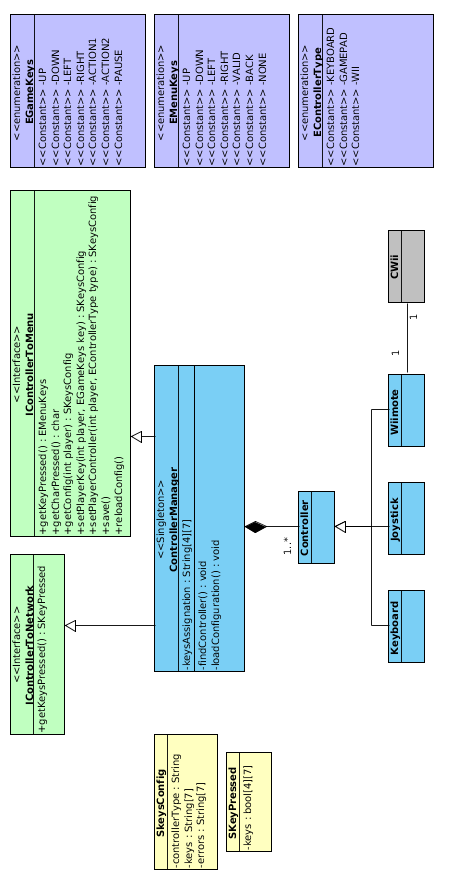
\includegraphics[angle=90]{images/UML/classDiagram/controller}
